% COntinued Chpater Implementation
\section{Content Based Model}
\label{sec:cb}

The content-based model uses vector space models of a user and an item to find the similarity between two vectors. The overview of content-based model is discussed in the \autoref{fig:content_based_flowchart}. 
\begin{singlespace}
\begin{figure}[H]
	\centering
	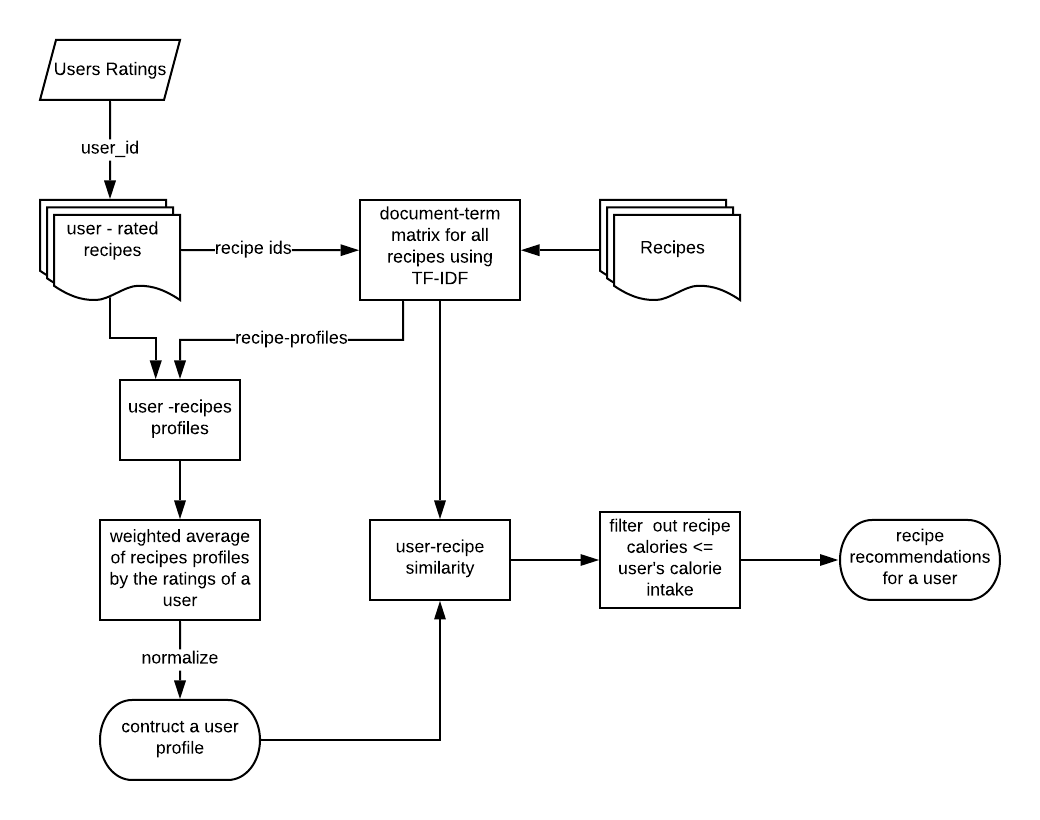
\includegraphics[width=1.0\linewidth]{content_based_flowchart}
	\caption{Content Based Filtering Work-Flow }
	\label{fig:content_based_flowchart}
\end{figure}  
\end{singlespace}

\noindent
All user interactions are denoted by 'Users Ratings' and all recipes information is denoted by 'Recipes'. Required steps to generated a user profile and a recipe profile are discussed below.
\begin{itemize}
\item All recipe profiles are generated based on the relevancy of terms to be considered. The term may vary based on the application area. In this thesis, ingredients, cooking methods, and diet labels are considered. The relevancy of terms in the documents is measured by TF-IDF as discussed in \nameref{sec:tf-idf}. A document term matrix is generated and stored for all recipes. 
\item Rated recipes for a single user are filtered from all user interactions.
Rated recipes are then filtered out and stored from a stored document-term matrix. 
\item To construct a user profile, recipes vectors rated by a user are considered. Then a weighted average of rated recipe profiles is calculated. The user profile is further normalized on the weighted values. 
\item Similarity between the user profile and all recipe profiles from the dataset is measured by cosine similarity as discussed in \nameref{cosine_similarity}. Recipes that are rated previously by the user are omitted to calculate relevance. Sort these recipes in descending order of similarity scores.
\item On the resultant recipes vectors we have applied a calorie intake filter comparing recipe calories and user required calories. These recipes are offered as recommendations to the user.  
\end{itemize}
 
\begin{singlespace}
\begin{figure}[H]
	\centering
	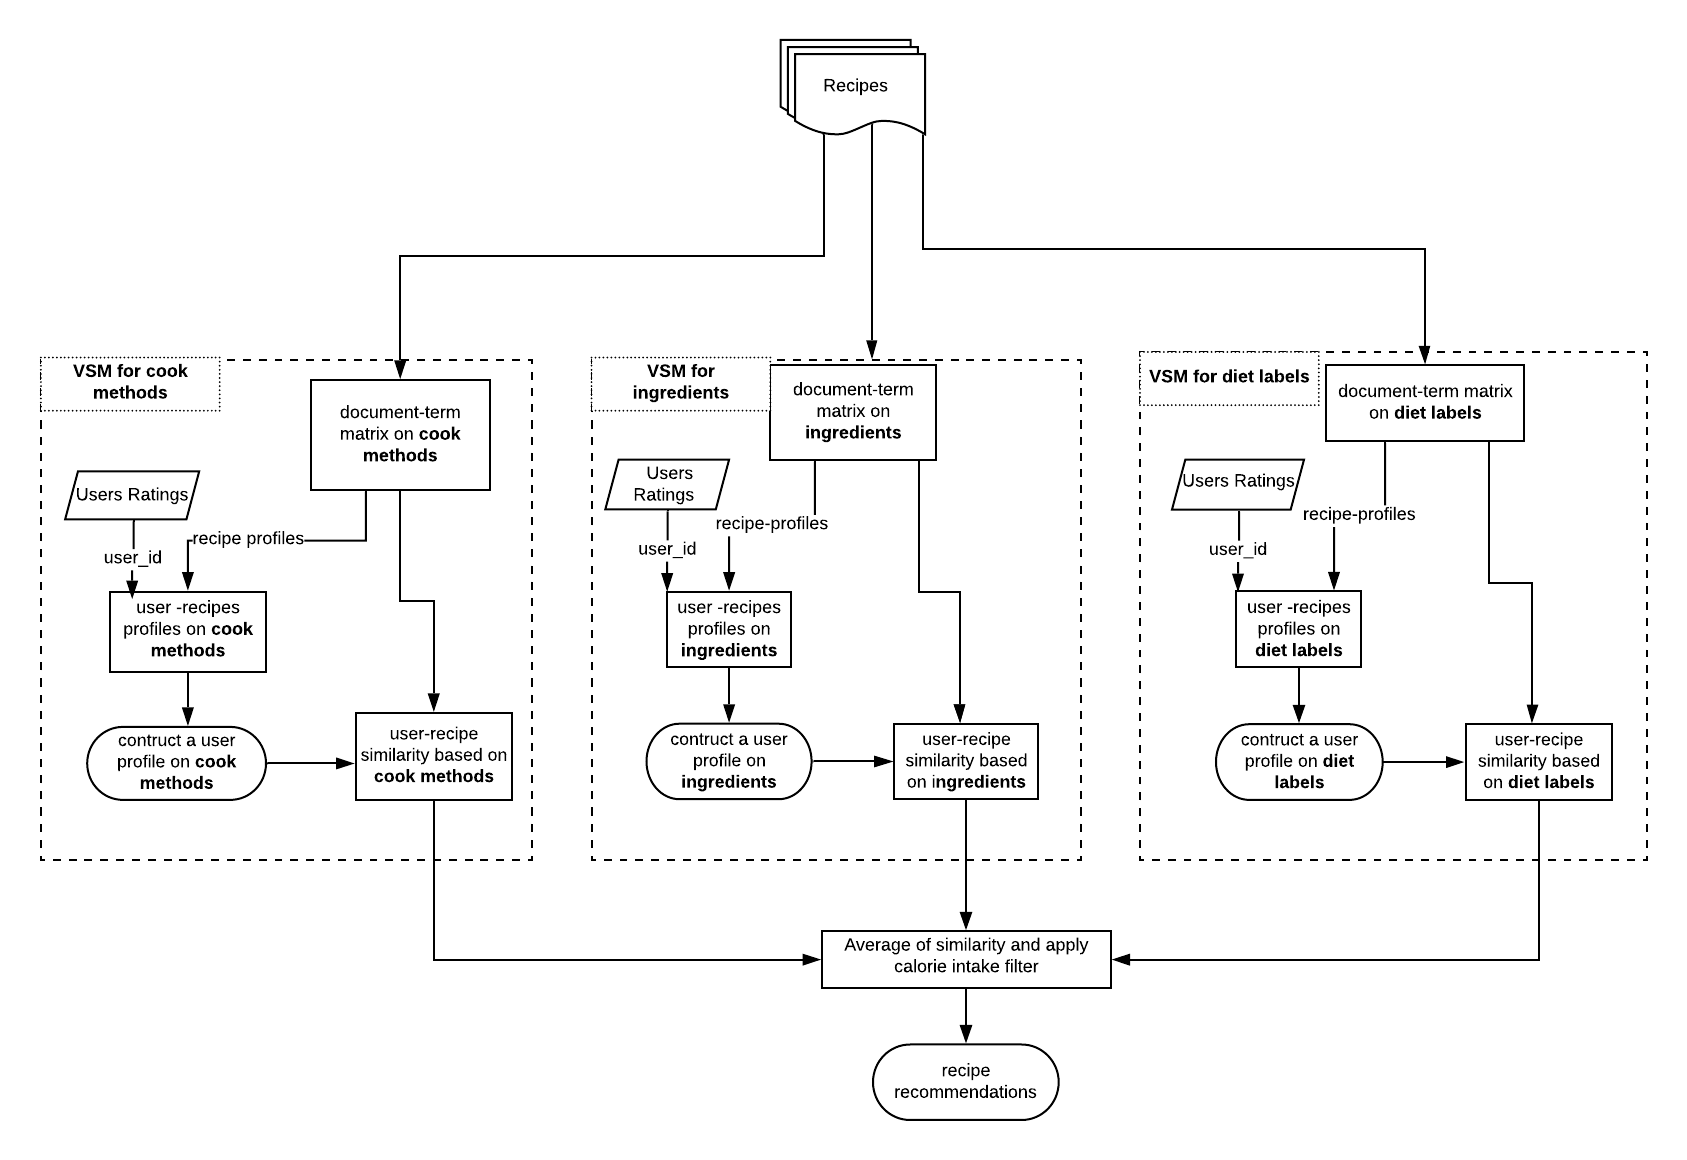
\includegraphics[width=1.25\linewidth]{content_based_ingredients_cookmethod_dietlabels}
	\caption{Content Based Filtering Combined Work-Flow }
	\label{fig:content_based_ingredients_cookmethod_dietlabels}
\end{figure}  
\end{singlespace}


\subsection{Content-Based Using Ingredients}
\label{sec:cb_ingredients}
Recipe ingredients are used to calculate recommendations in content-based using ingredients approach. The user profile and recipe profiles are generated using ingredients in the recipes. The steps to generate recommendations for a user using ingredients in content based model are discussed below.
\begin{itemize}
\item All ingredients from recipes are extracted. 
\item Similarity between recipes are considered based on ingredients but there are many ingredients are commonly used in all recipes such as salt. To get the importance of ingredients which are relevant to the recipe and to negate effect of high frequency terms, concept of TF-IDF has been used as discussed in \nameref{sec:tf-idf}. The recipe vector or recipe profile is calculated for each recipe in the dataset. The 'TfidfVectorizer' function from 'sklearn' has been used to calculate TF-IDF.
\item The weighted average of a user rated recipe profiles is calculated to construct a user profile. Constructed user profile is based on ingredients of the recipes.  
\item Similarity between a user profile and all recipe profiles in the dataset is calculated using cosine similarity. The 'linear\_kernel' function from the 'sci-kit learn' library has been used for the same. 
\item The resultant profiles are listed in descending order of similarity score to get more relevant recipes at top. At this point recipes already rated by a user are omitted. 
\item From user's information, the BMR and the required calorie intake per meal is calculated. 
\item The resultant set of recipes are offered as recommendations. 
\end{itemize}
\subsubsection{Experiment}
\label{sec:cb_ingred_exp}
The purpose of this experiment was to evaluate the user recommendations on Ingredients algorithm mentioned in the \nameref{sec:cb_ingredients}. For this experiment, \lq{}Ingredients\rq{} attribute is used that is described in the section \nameref{sec:data_prep}. The training and testing datasets are split as explained in the section \nameref{sec:traintest}. The experiment was performed for an output set of 5, 10 and 20 recommendations. 

\subsection{Recommendations Using Ingredients and Cook Methods}
\label{sec:cb_ingredients_cook_method}
\subsubsection{Experiment}
\label{sec:cb_ingred_cook_method_exp}
The purpose of this experiment was to evaluate the user recommendations on ingredients and cook method  algorithm mentioned in the \nameref{sec:cb_ingredients_cook_method}. For this experiment, \lq{}Ingredients\rq{} and \lq{}Cook Method\rq{} attributes are used that are described in the section \nameref{sec:data_prep}. The training and testing datasets are split as explained in the section \nameref{sec:traintest}. The experiment was performed for an output set of 5, 10 and 20 recommendations. 

\subsection{Recommendations Using Ingredients, Cooking Method and Diet Labels}
\label{sec:cb_ingredients_cook_method_diet_labels}
\subsubsection{Experiment}
\label{sec:cb_ingred_cook_method_diet_label_exp}
The purpose of this experiment was to evaluate the user recommendations on ingredients, cook method  and diet labels algorithm mentioned in the \nameref{sec:cb_ingredients_cook_method_diet_labels}. For this experiment, \lq{}Ingredients\rq{}, \lq{}Cook Method\rq{} and \lq{}Diet Label\rq{} attributes are used that are described in the section \nameref{sec:data_prep}. The training and testing datasets are split as explained in the section \nameref{sec:traintest}. The experiment was performed for an output set of 5, 10 and 20 recommendations. 